\section{Проверка гипотез}

Для того, чтобы проверить выдвинутые гипотезы, я построил и проанализировал 12 графиков: на каждом наборе данных (результаты опросов школьников и администрации) я применил алгоритмы UMAP и PCA, а потом сравнил их результаты.
Интересно, что распределения у студентов, полученные с помощью PCA и UMAP, практически не отличаются друг от друга, в то время как распределение ответов администрации может меняться в зависимости от того, какую целевую переменную мы предсказываем.
Этот эффект объясняется тем, что я использовал две различные техники кластеризации в процессе работы с данными.
В случае администрации, я выделял целевую переменную, оставшиеся кодировал, нормализировал, а потом понижал размерность.
В случае же ответов учеников, я заранее определил набор целевых переменных, по которым буду различать результаты эксперимента, и понижал размерность оставшихся данных.

\subsection{Распределение ответов на опрос не зависит от гендера участников} \label{hypothesis::1}

\begin{figure}[h!]
    \centering
    
    \begin{subfigure}{.5\textwidth}
      \centering
      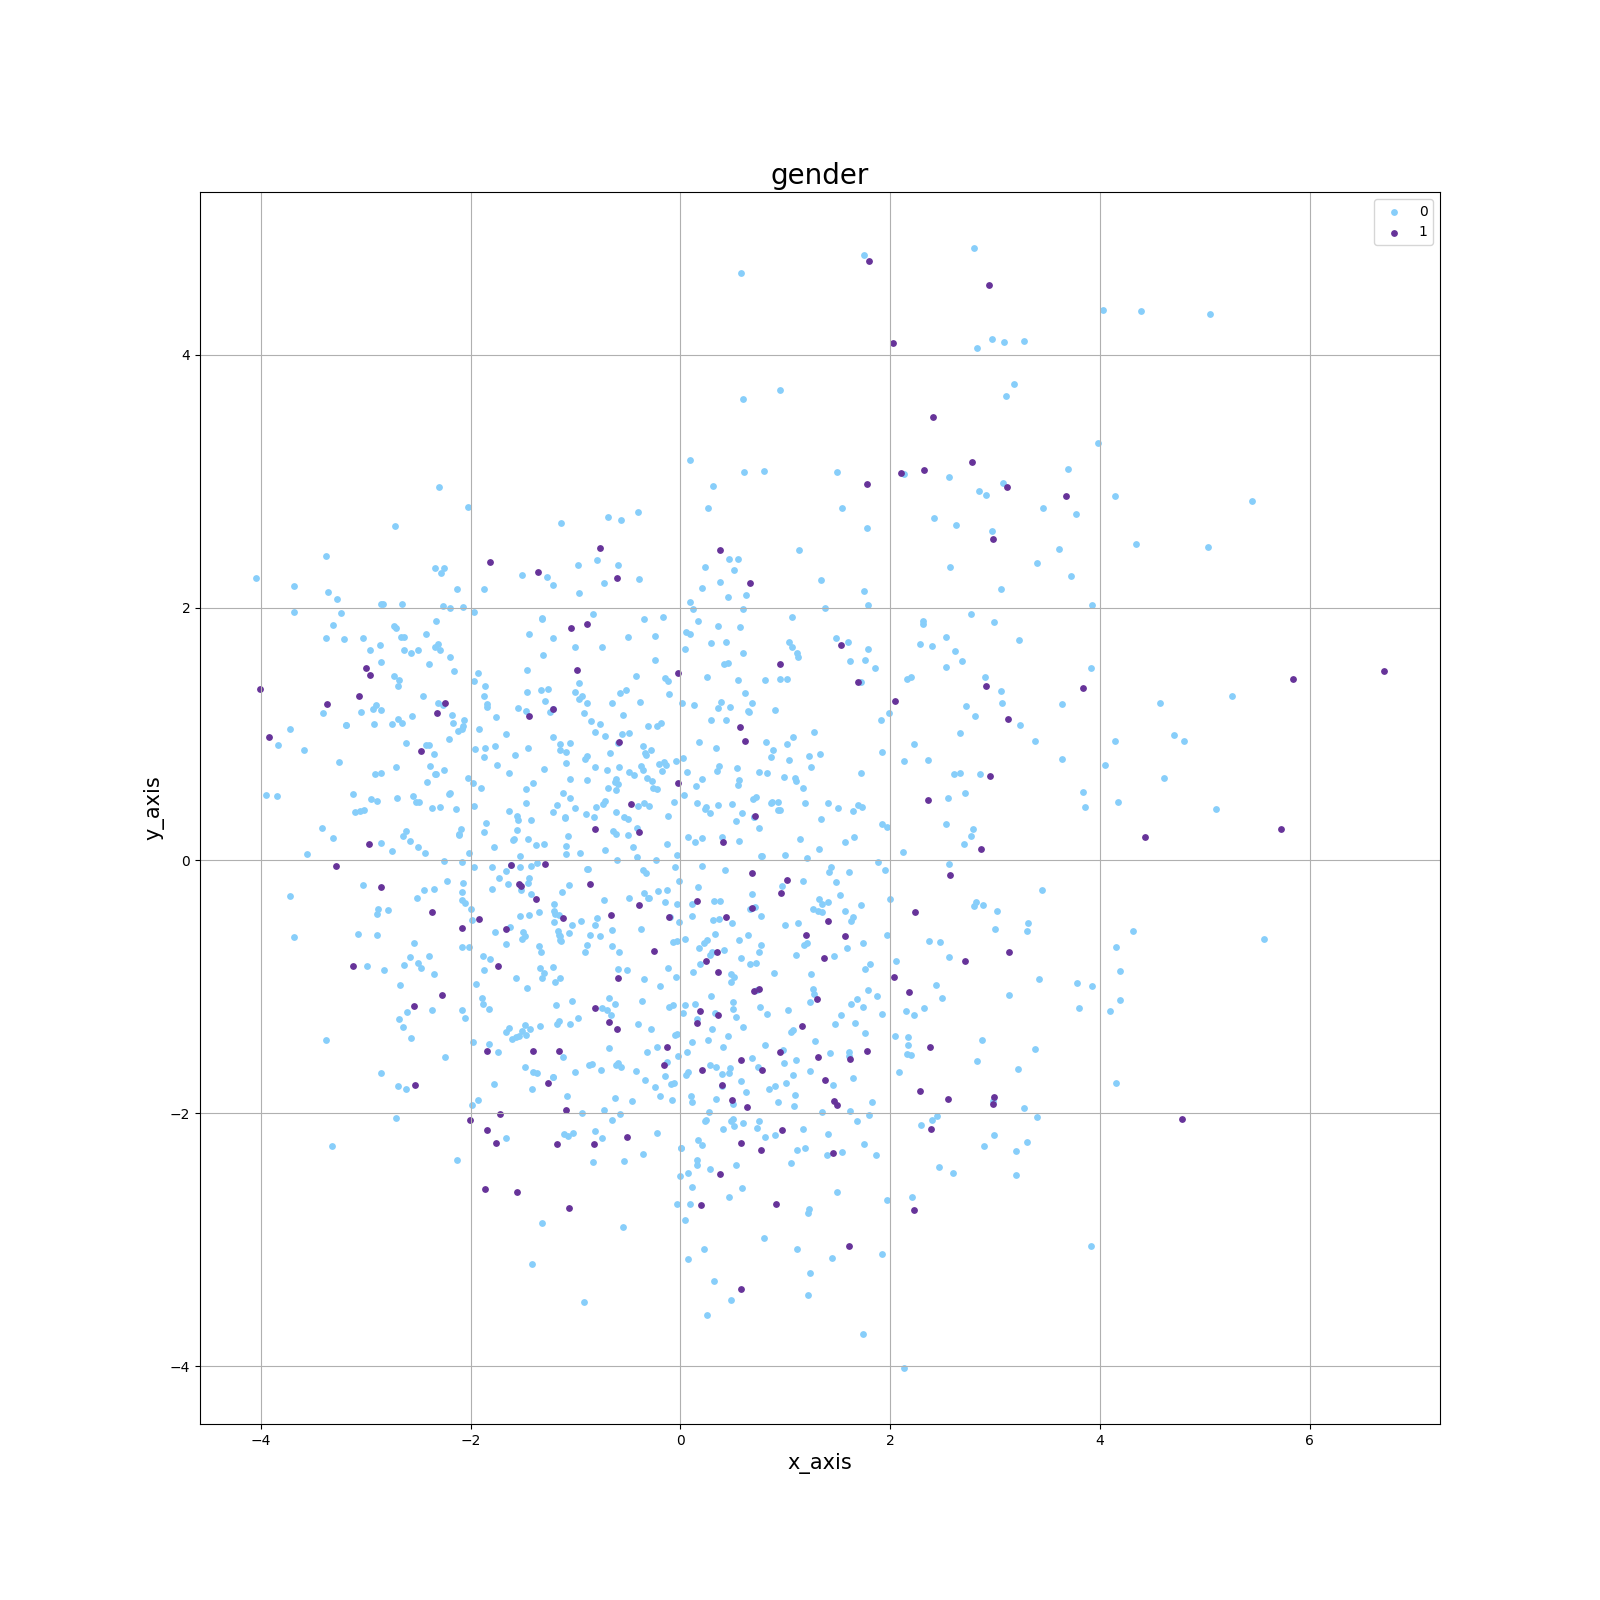
\includegraphics[width=\linewidth]{../img/administration_PCA_gender.png}
      \caption{PCA}
      \label{img::administration::gender::PCA}
    \end{subfigure}%
    \begin{subfigure}{.5\textwidth}
      \centering
      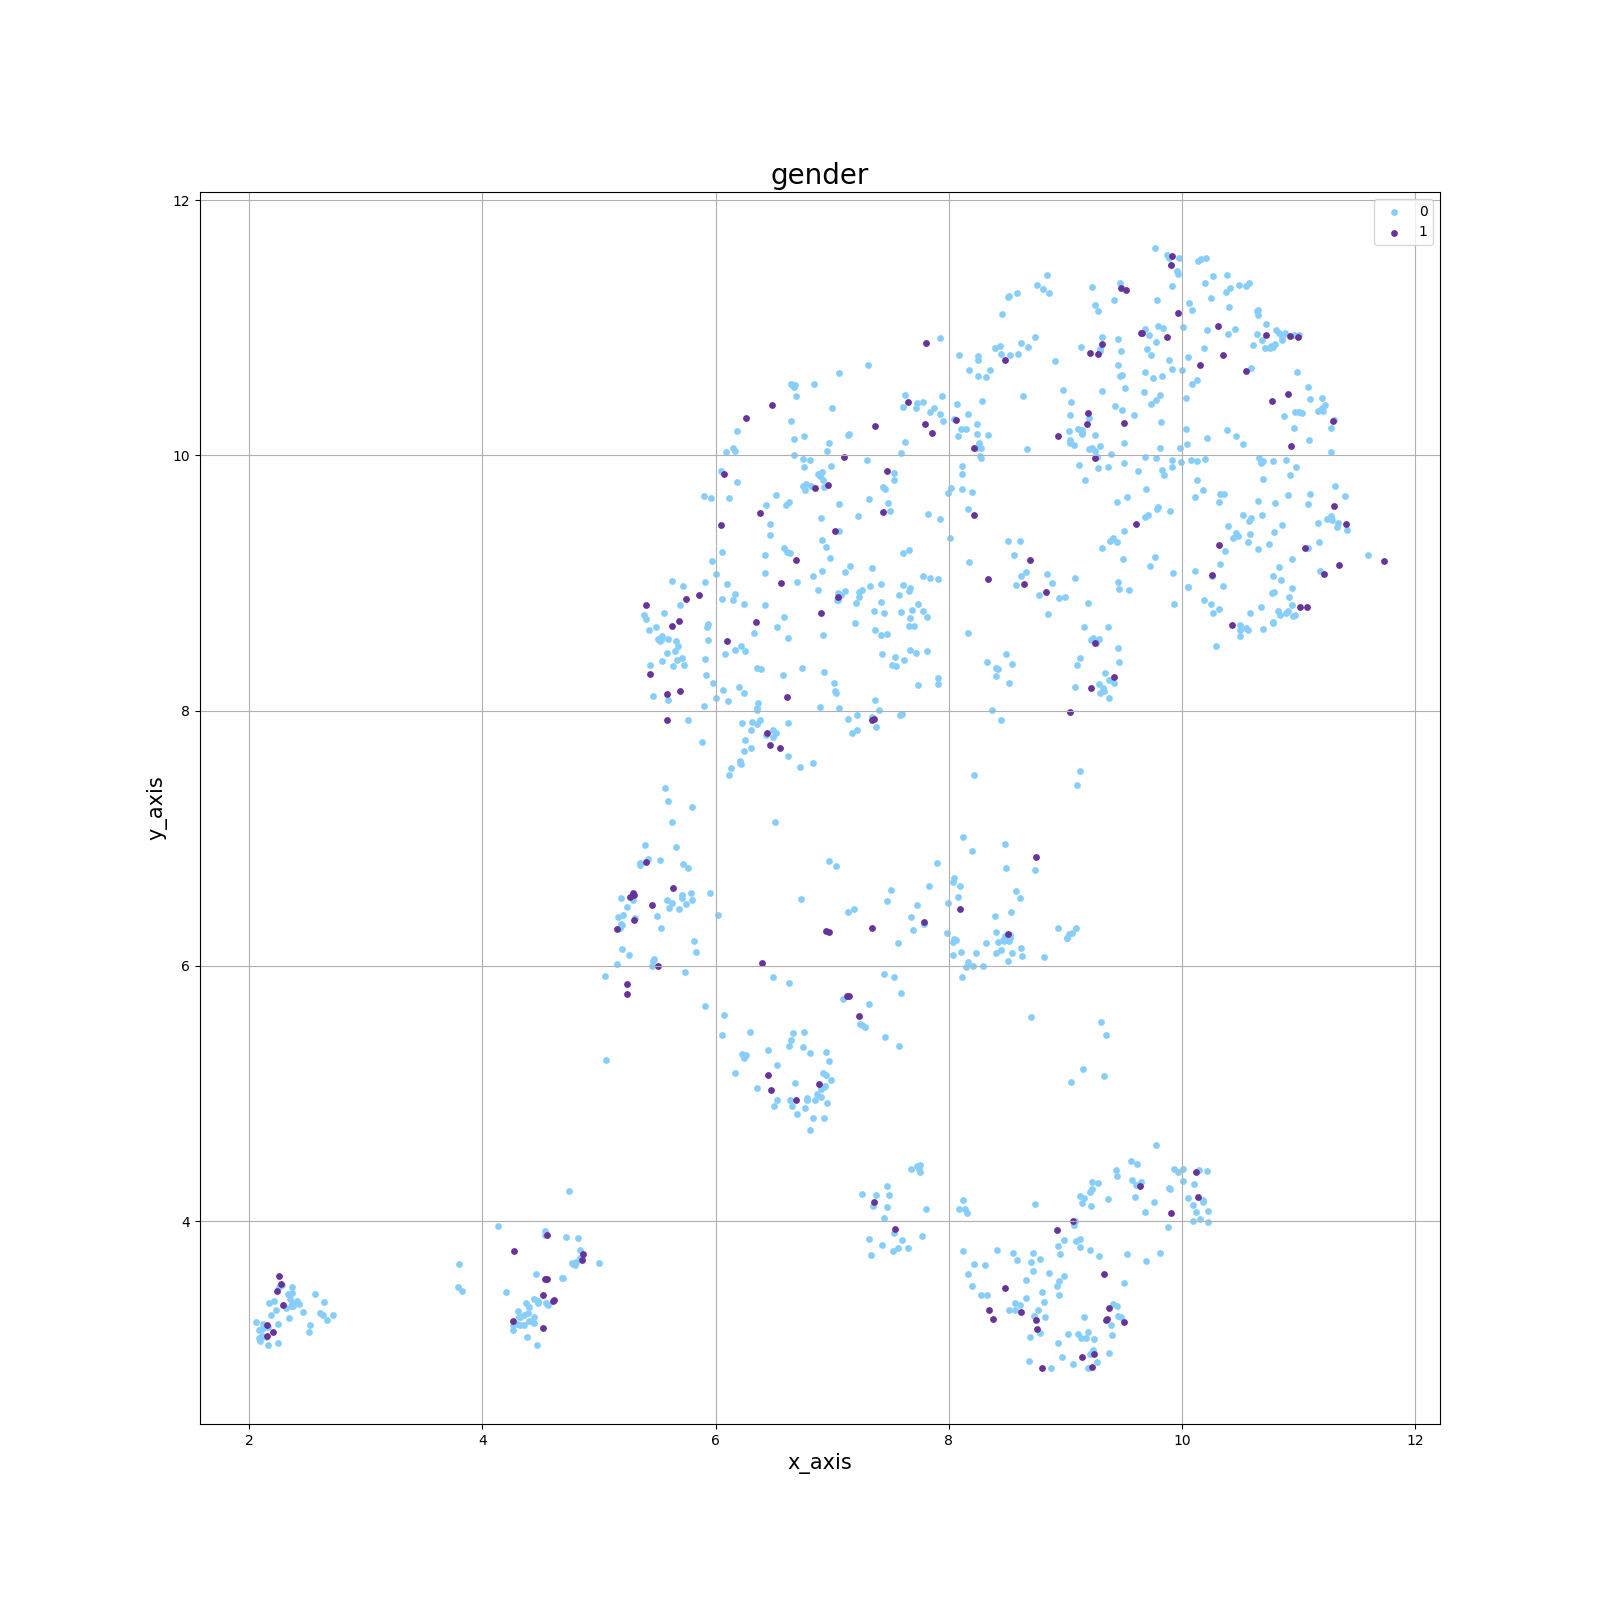
\includegraphics[width=\linewidth]{../img/administration_UMAP_gender.png}
      \caption{UMAP}
      \label{img::administration::gender::UMAP}
    \end{subfigure}
    \caption{Распределение ответов администрации в зависимости от пола}
\end{figure}

На построенных распределениях для администрации (рис. \ref{img::administration::gender::PCA} и \ref{img::administration::gender::UMAP}) мы можем видеть, что вне зависимости от гендера респондентов, распределяются по кластерам они примерно одинаково, с той лишь разницей, что женского персонала в составе администрации школ сильно больше, чем мужского.
Аналогичное распределение мы можем наблюдать и на ответах школьников (рис. \ref{img::students::gender::PCA} и \ref{img::students::gender::UMAP}), только в этом случае у нас примерно одинаковое количество респондентов разного пола.
Таким образом, гипотеза подтверждается, ответы участников действительно не зависят от пола.

\begin{figure}[h!]
    \centering
    
    \begin{subfigure}{.5\textwidth}
      \centering
      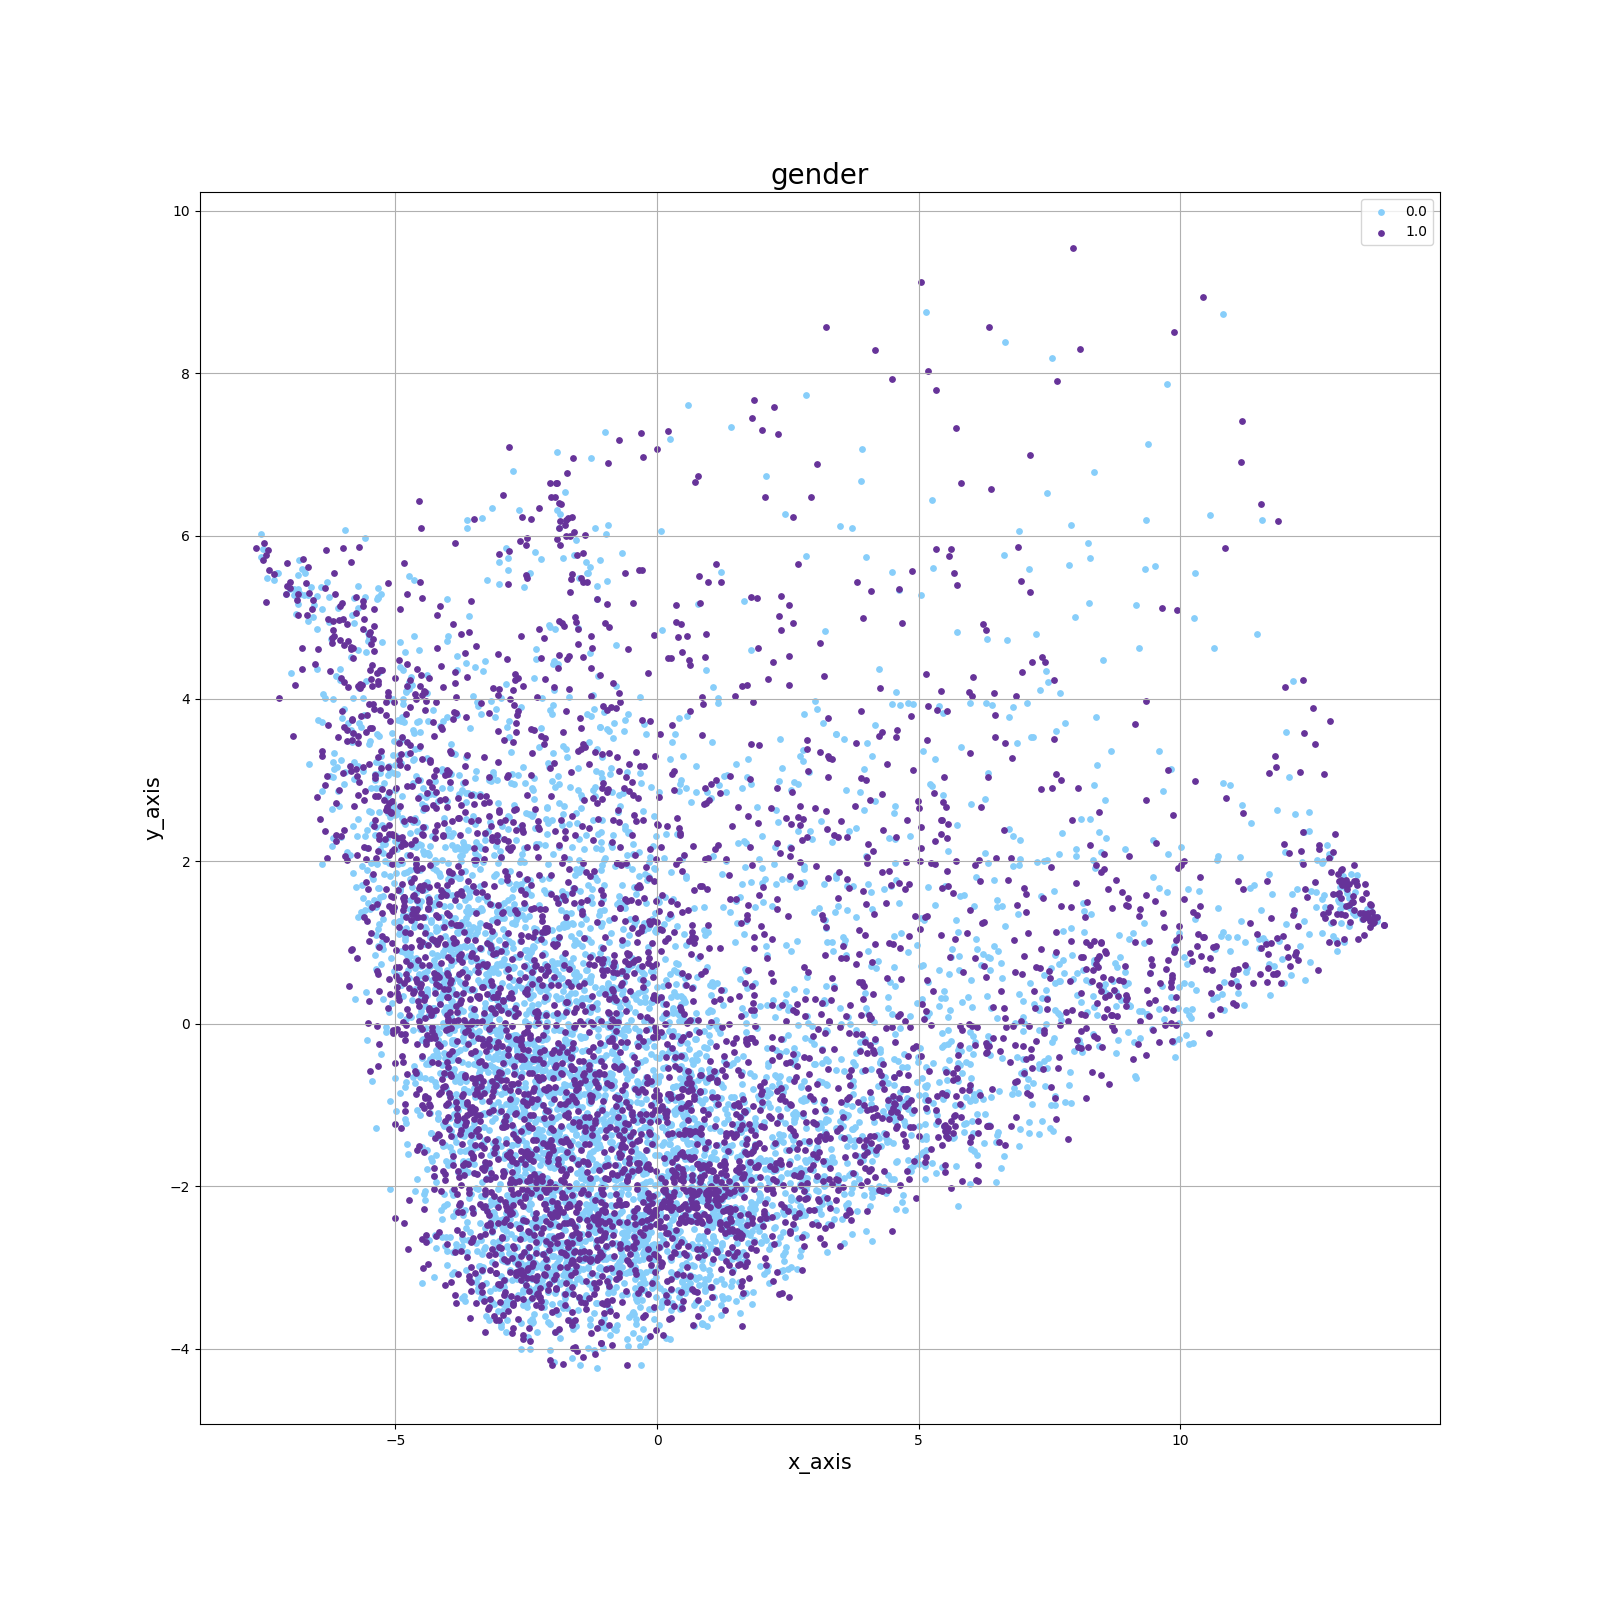
\includegraphics[width=\linewidth]{../img/students_PCA_gender.png}
      \caption{PCA}
      \label{img::students::gender::PCA}
    \end{subfigure}%
    \begin{subfigure}{.5\textwidth}
      \centering
      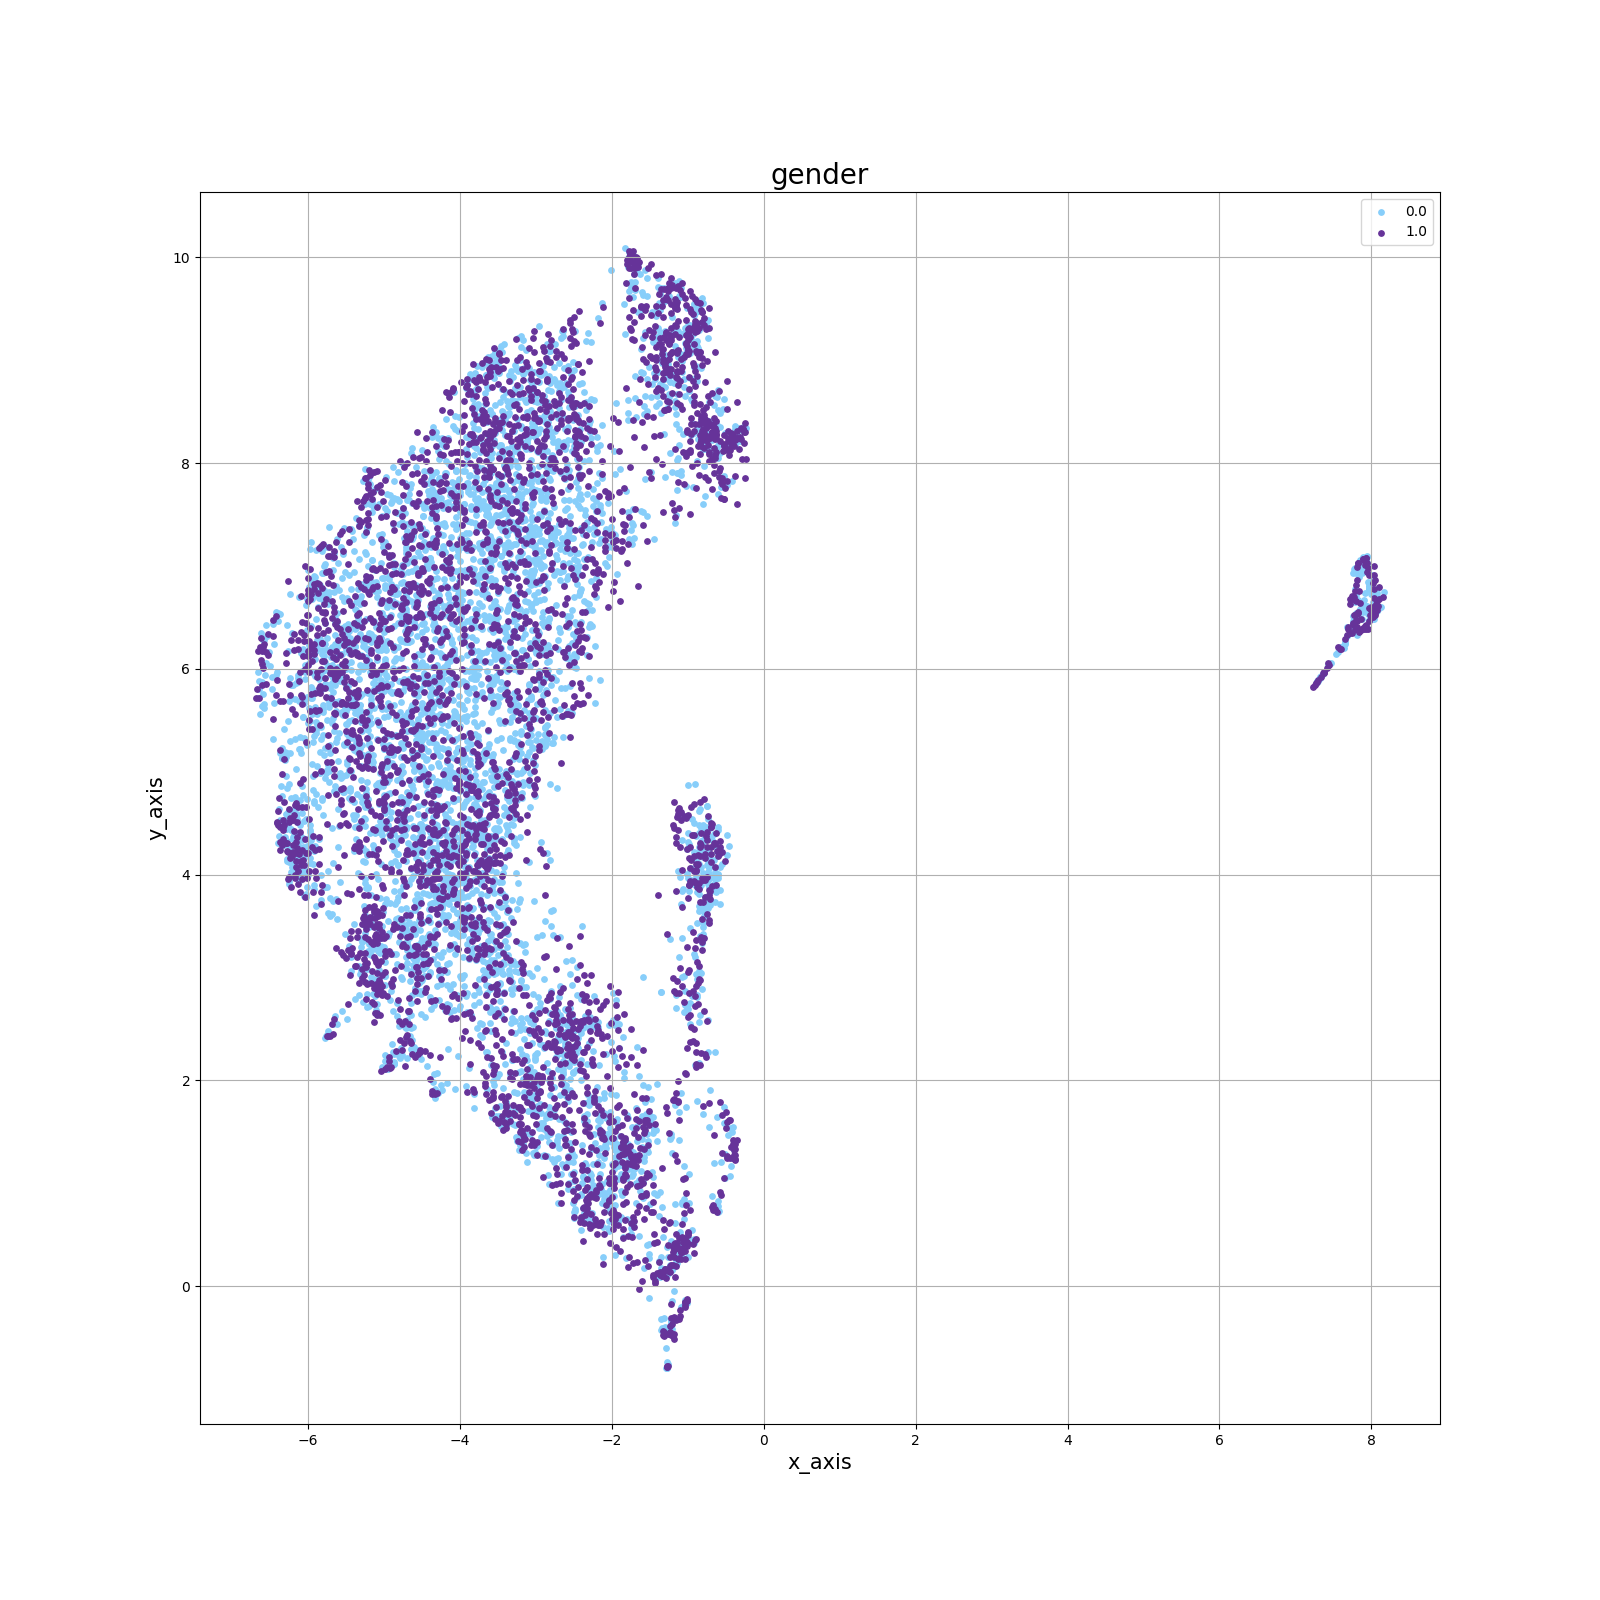
\includegraphics[width=\linewidth]{../img/students_UMAP_gender.png}
      \caption{UMAP}
      \label{img::students::gender::UMAP}
    \end{subfigure}
    \caption{Распределение ответов школьников в зависимости от пола}
\end{figure}

\subsection{Распределение ответов учеников на опрос не зависит от класса, в котором ученик обучается}

\begin{figure}[H]
    \centering
    \begin{subfigure}{.5\textwidth}
      \centering
      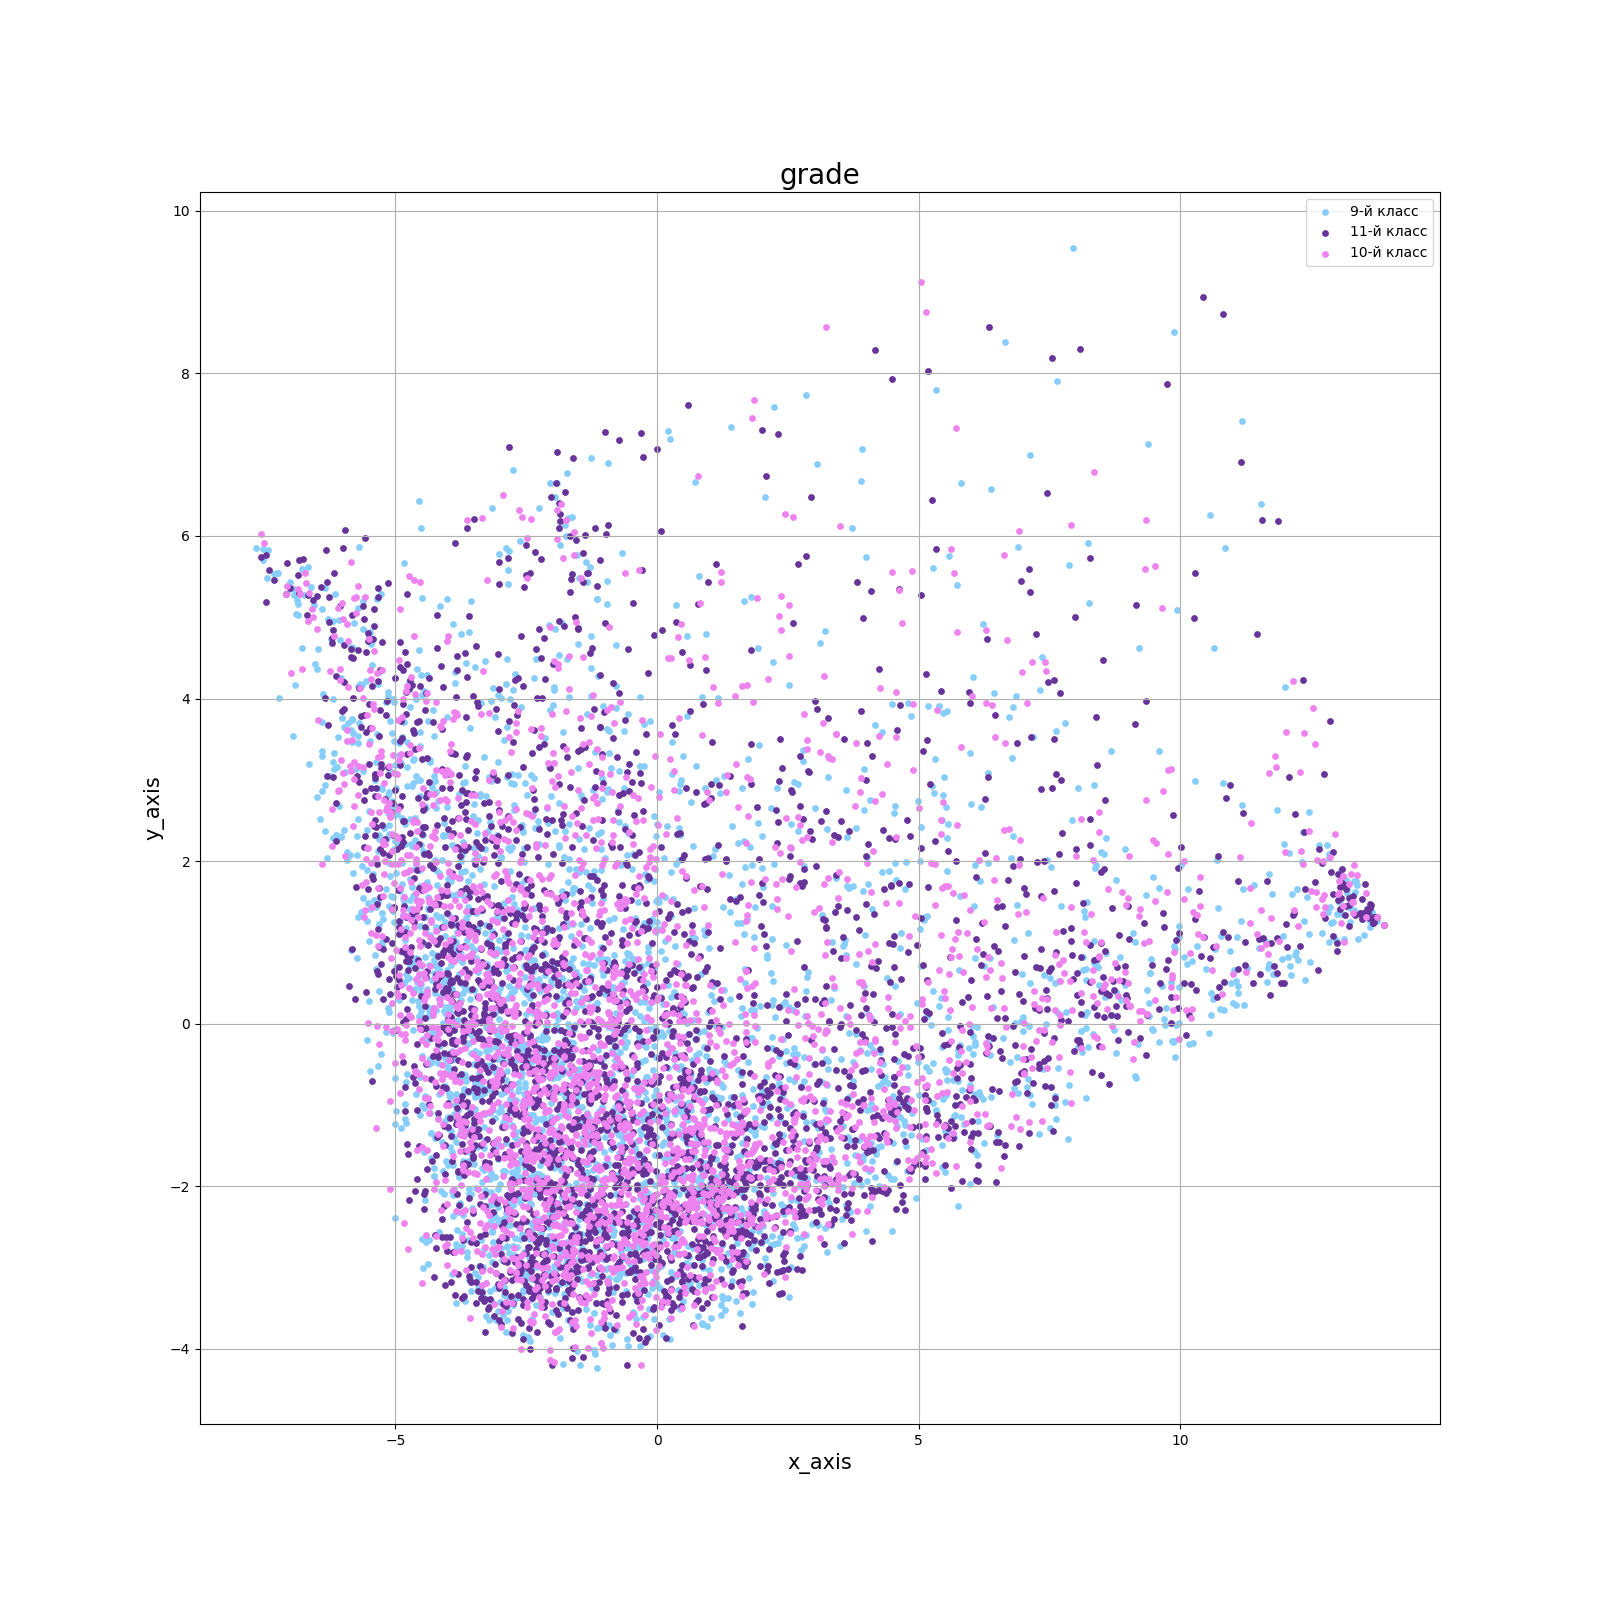
\includegraphics[width=\linewidth]{../img/students_PCA_grade.png}
      \caption{PCA}
      \label{img::students::grade::PCA}
    \end{subfigure}%
    \begin{subfigure}{.5\textwidth}
      \centering
      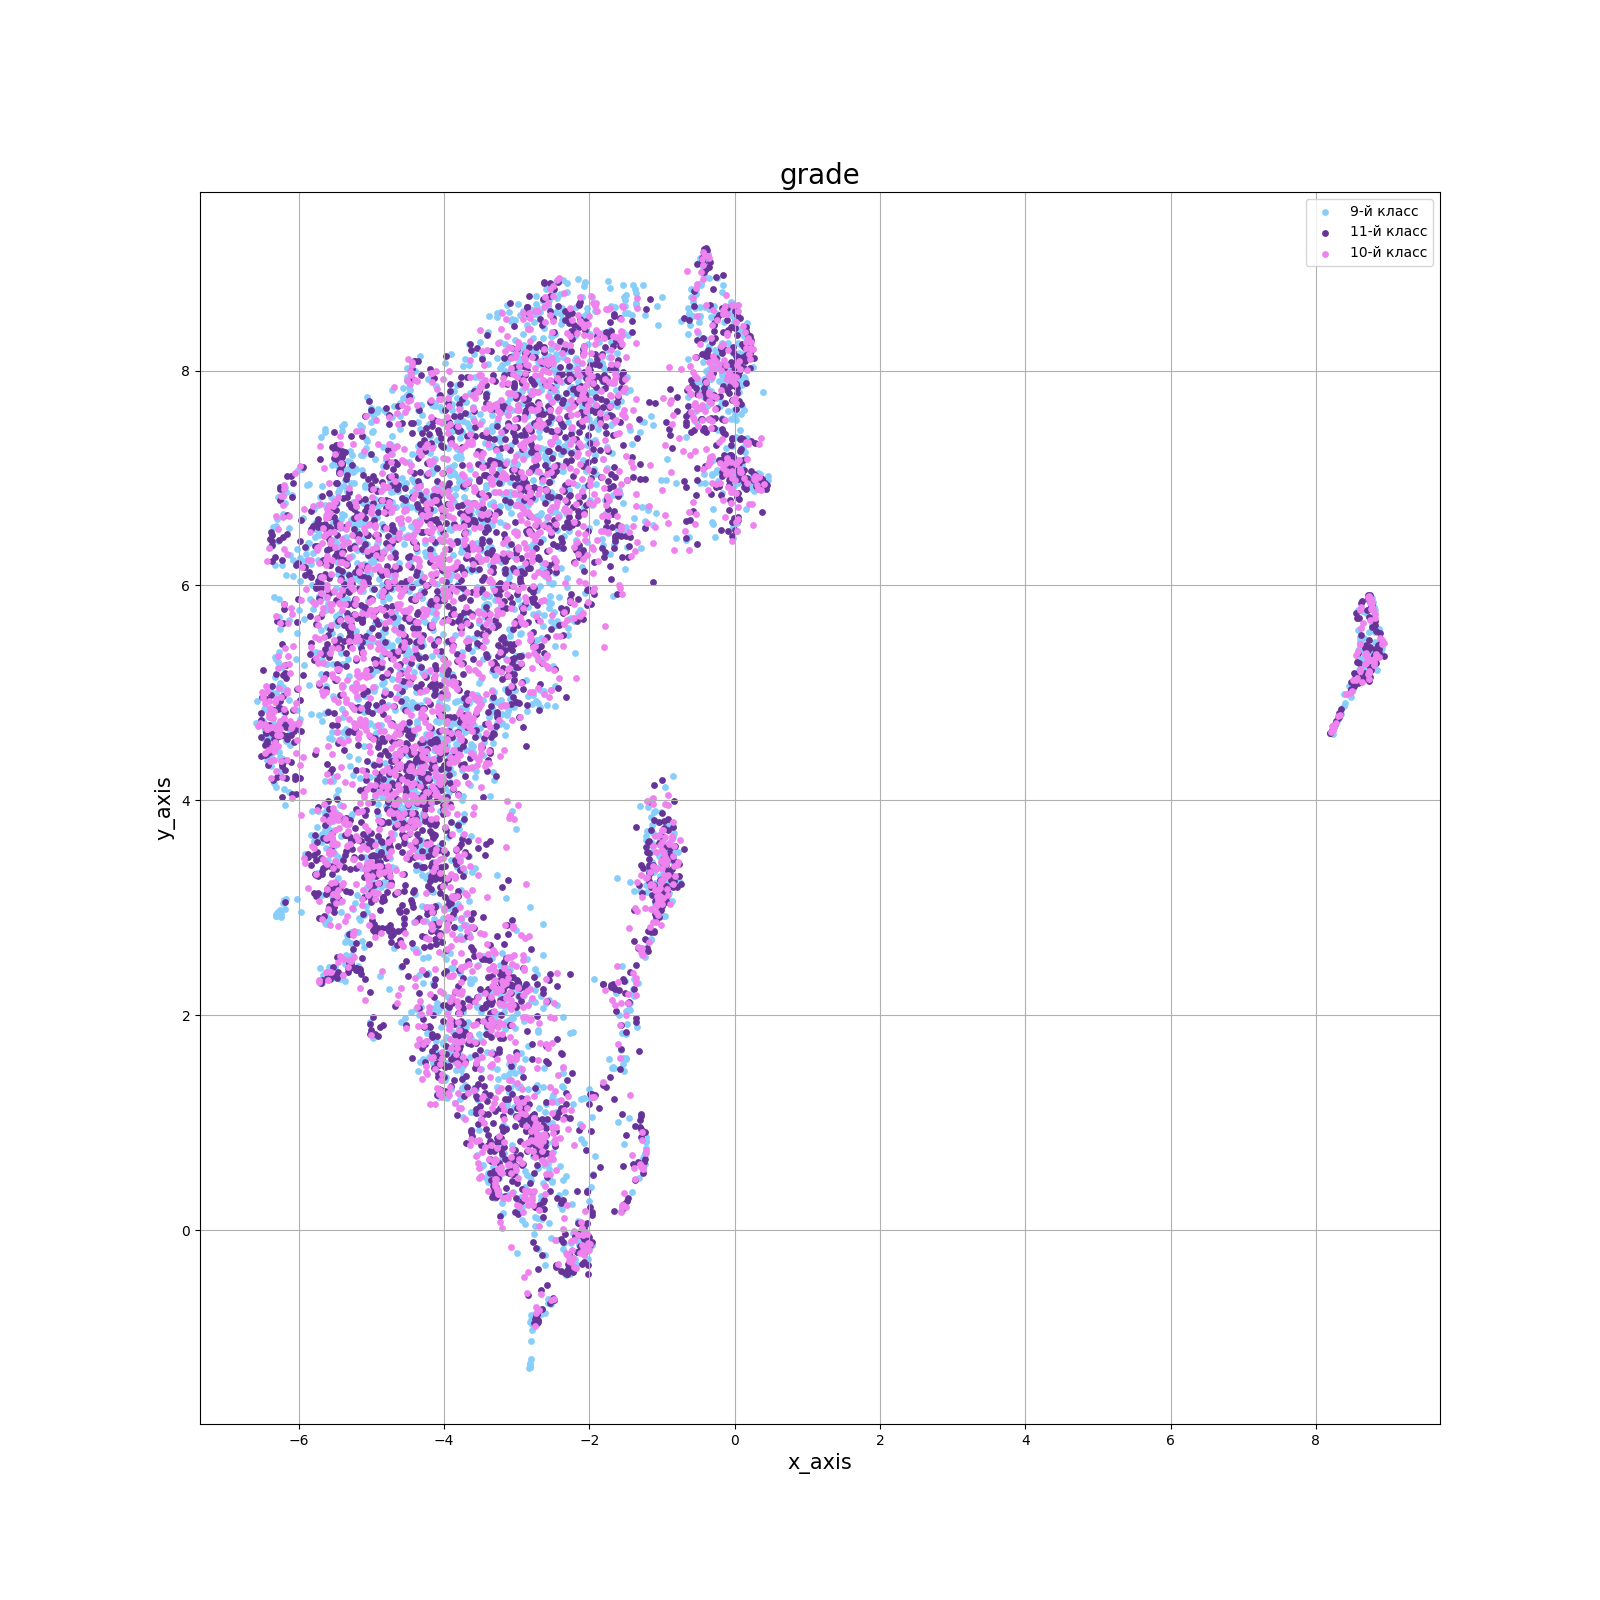
\includegraphics[width=\linewidth]{../img/students_UMAP_grade.png}
      \caption{UMAP}
      \label{img::students::grade::UMAP}
    \end{subfigure}
    \caption{Распределение ответов студентов в зависимости от класса}
\end{figure}

На рис. \ref{img::students::grade::PCA} и \ref{img::students::grade::UMAP} мы можем заметить две вещи:
\begin{enumerate}
    \item Распределение абсолютно не отличается от того, которое было в секции \ref{hypothesis::1}, что не удивительно, учитывая тот факт, что я просто подменил целевую переменную, по которой раскрашиваю точки в пространстве.
    \item Распределение по классам весьма равномерное в двух кластерах в случае рис. \ref{img::students::grade::UMAP}.
\end{enumerate}
Таким образом, класс учеников не влияет на их ответы в опросе про техническую оснащенность школы.
Это, на самом деле, весьма логично, ведь если школа использует IT технологии в образовательном процессе отдельной параллели, то она будет эти же технологии распространять и на все остальные параллели.

\subsection{Распределение ответов членов школьной администрации зависит от должности}

\begin{figure}[H]
    \centering
    
    \begin{subfigure}{.5\textwidth}
      \centering
      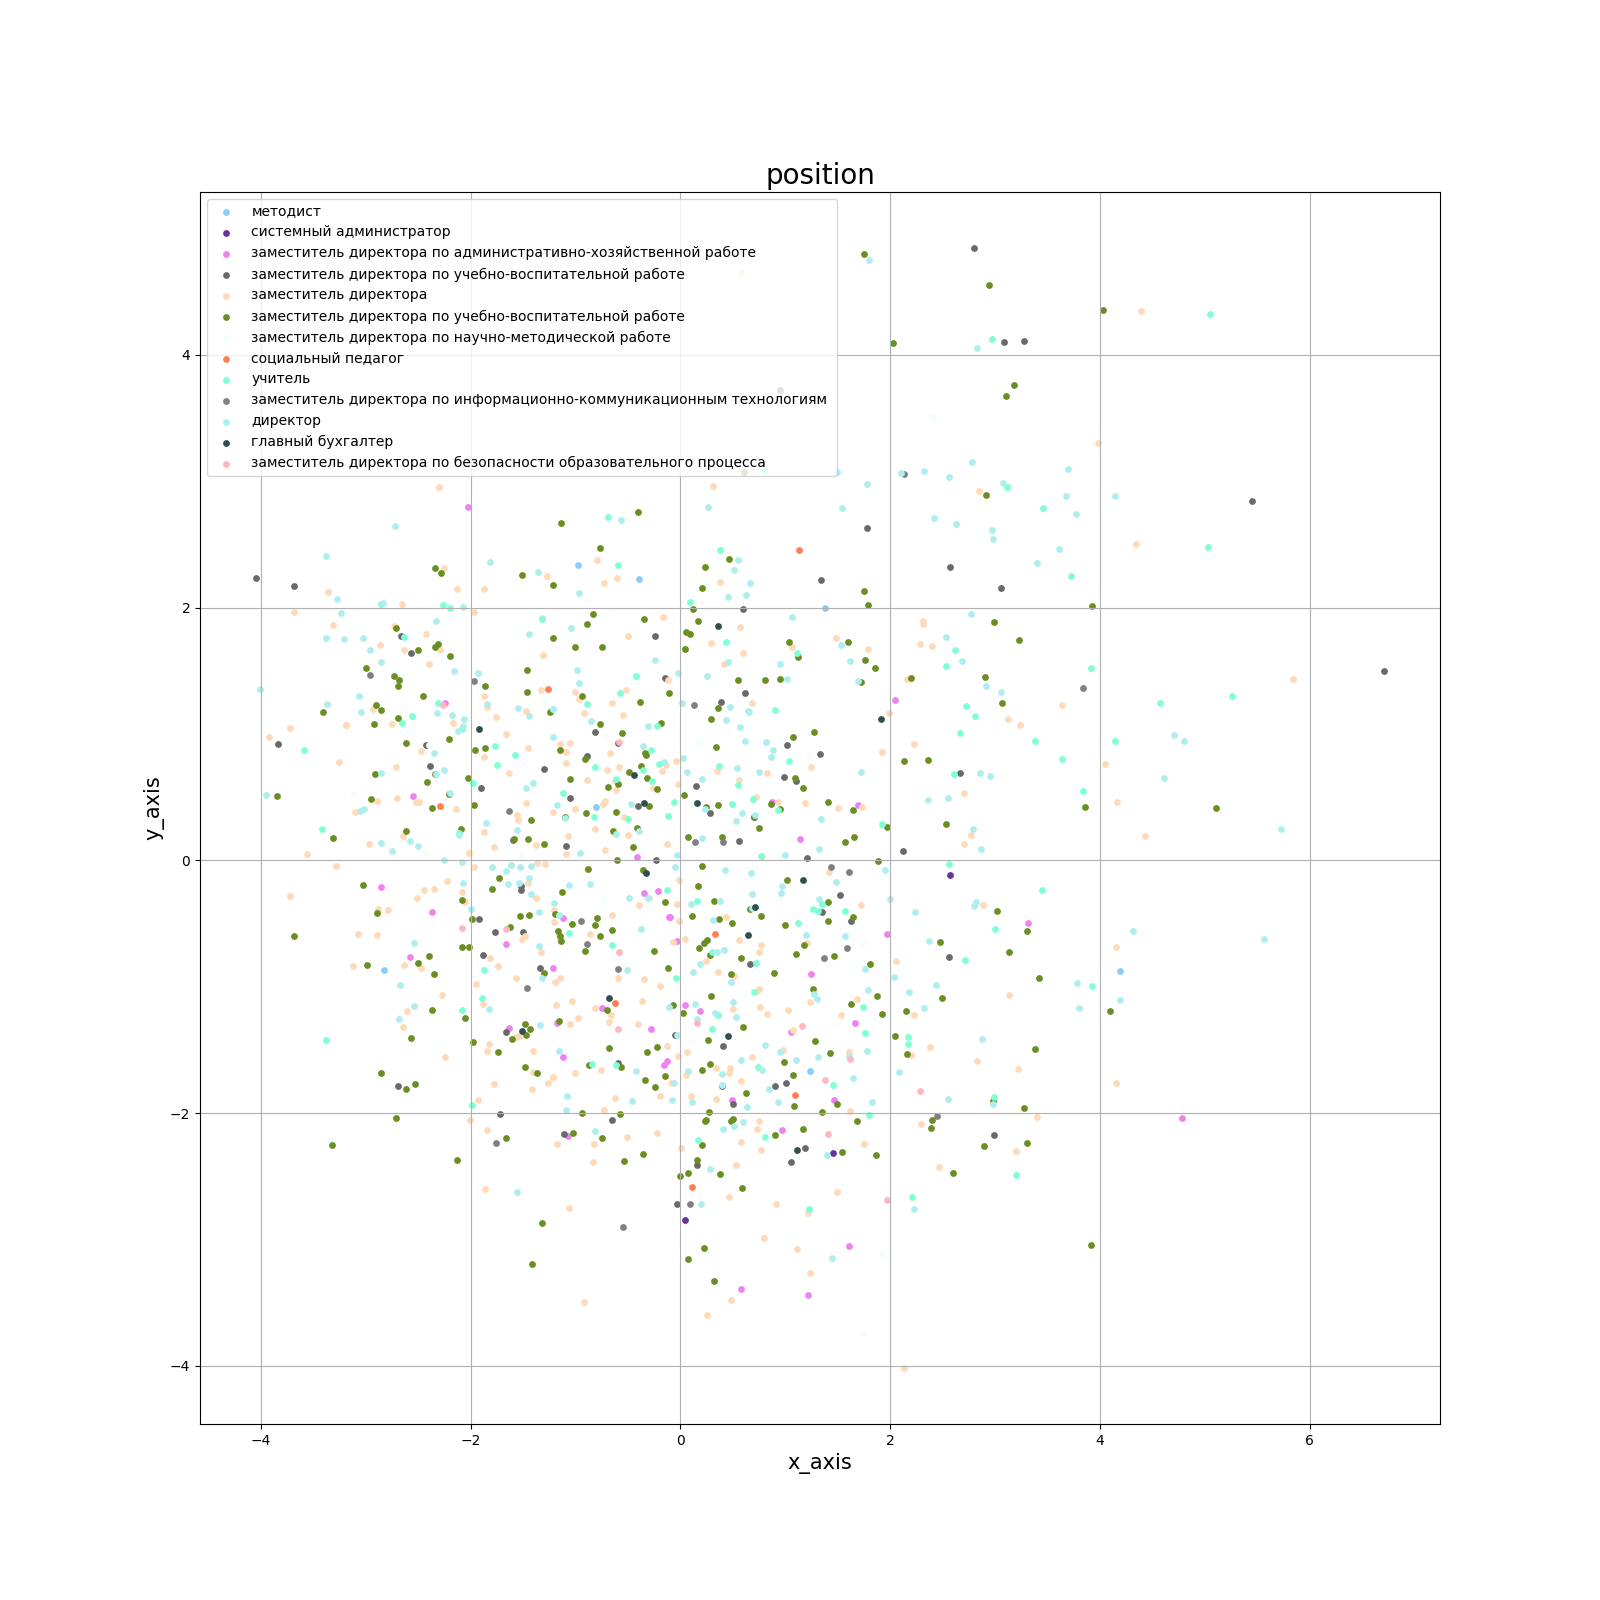
\includegraphics[width=\linewidth]{../img/administration_PCA_position.png}
      \caption{PCA}
      \label{img::administration::position::PCA}
    \end{subfigure}%
    \begin{subfigure}{.5\textwidth}
      \centering
      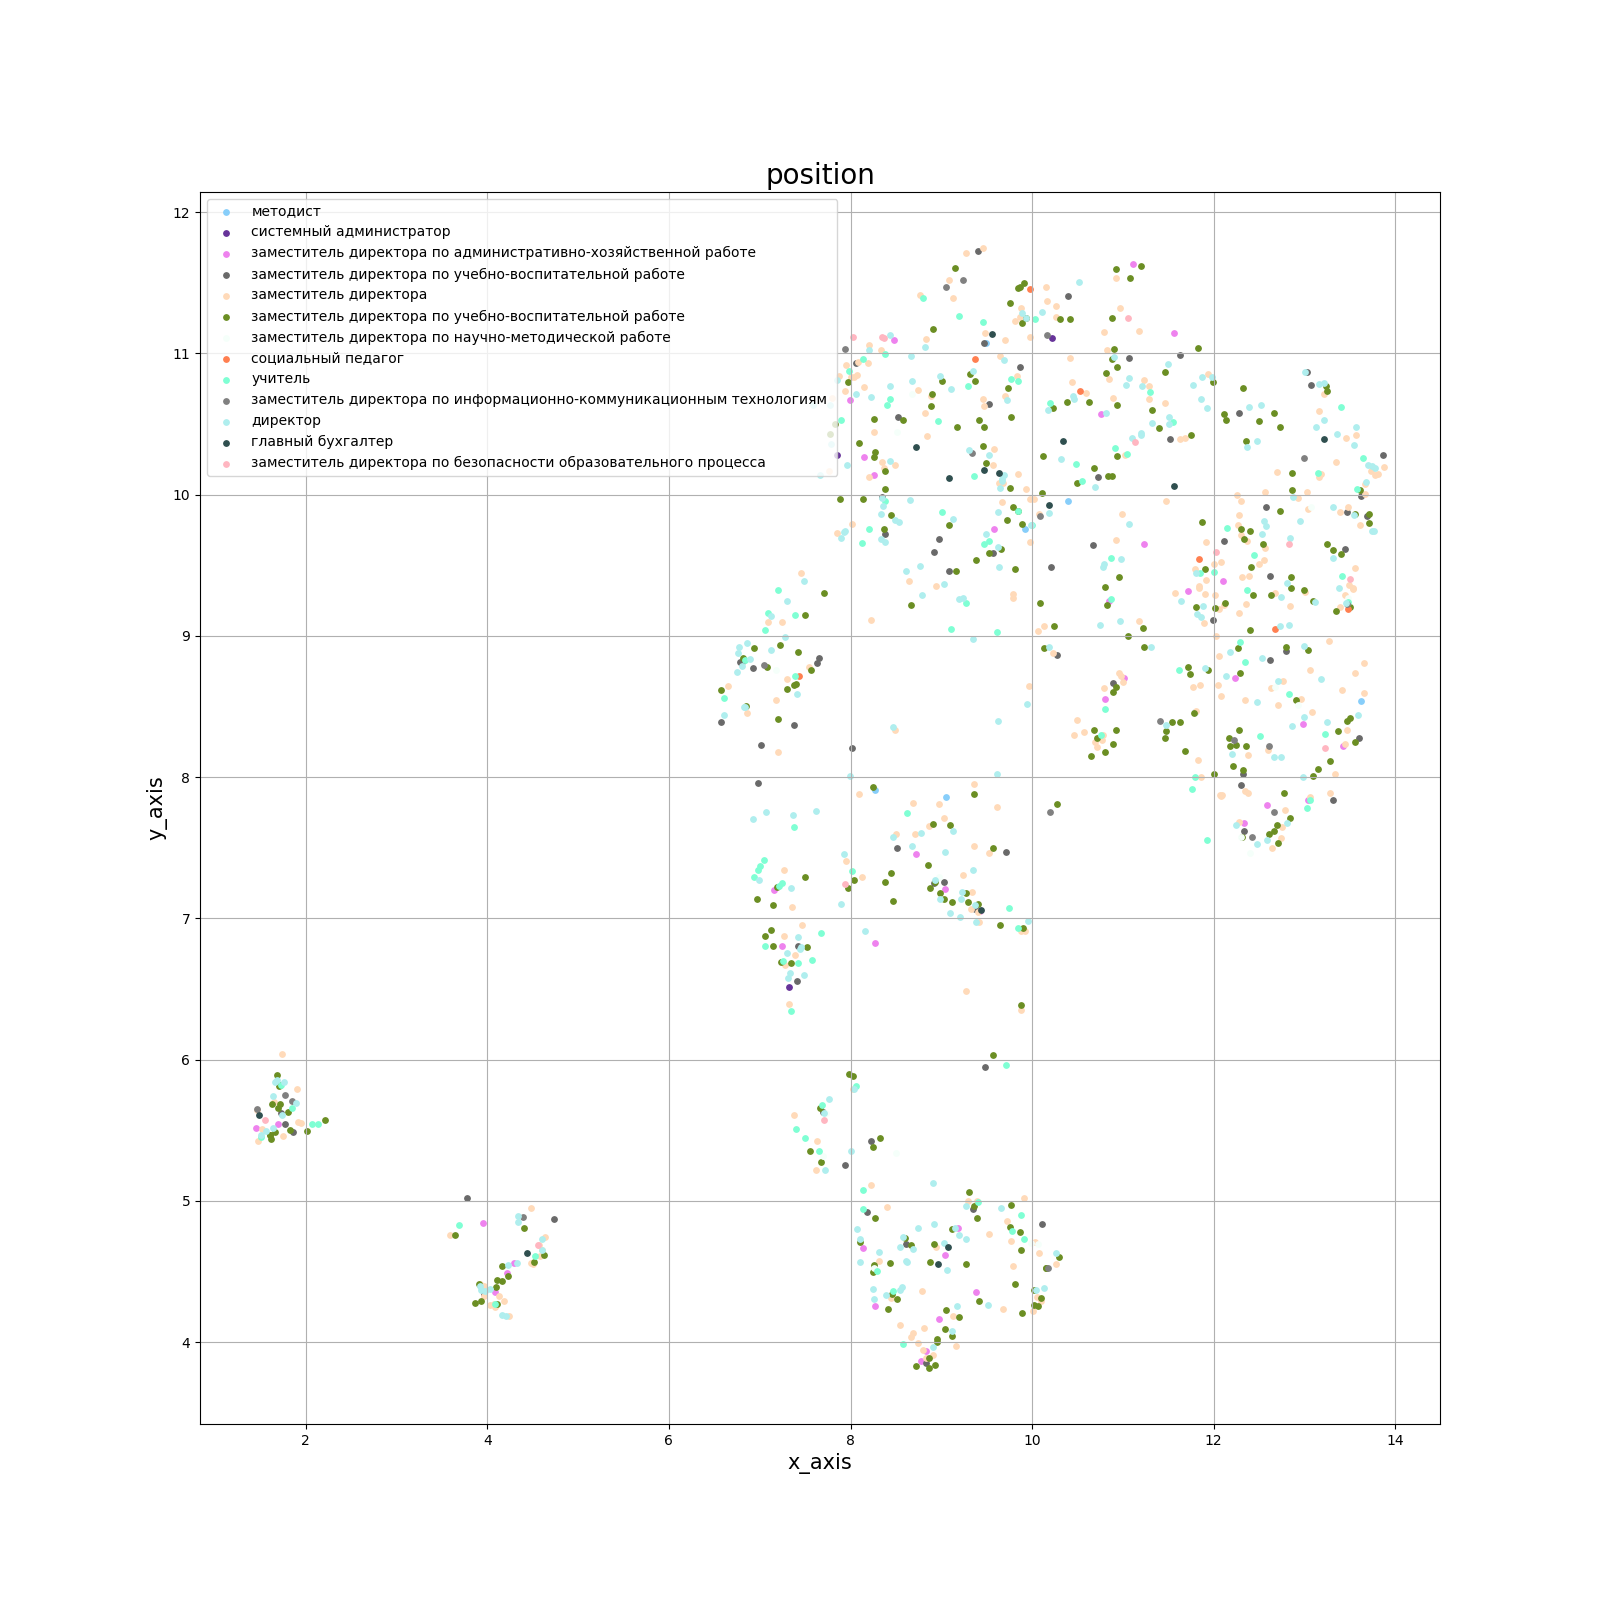
\includegraphics[width=\linewidth]{../img/administration_UMAP_position.png}
      \caption{UMAP}
      \label{img::administration::position::UMAP}
    \end{subfigure}
    \caption{Распределение ответов администрации школы в зависимости от должности}
\end{figure}

Как мы можем наблюдать, моя гипотеза не подтвердилась, поскольку почти все должности присутствуют в каждом из полученных кластеров на рис. \ref{img::administration::position::PCA} и \ref{img::administration::position::UMAP}.
Это говорит, как я предполагаю, о широкой осведомленности почти каждого сотрудника школьной администрации о технологической оснащенности школы.

\newpage
\section{План дальнейшей работы}

Следующей задачей является задача классификации респондентов в зависимости от их ответов.
Я попробую предсказывать школу человека по его ответам в опросе.
Также, в процессе предварительной обработки данных, я выбросил некоторые неструктурированные данные.
В частности, я проигнорировал все ответы на вопрос про использование конкретных электронных образовательных систем, хотя мне кажется, что в этих данных могут быть какие-то интересные закономерности.
Эти данные сложно поддаются обработке, однако я все равно попробую их почистить и по ним покластеризовать ответы участников опроса.

Также, планируется перебрать абсолютно все категориальные признаки, чтобы выявить, какой именно среди них влияет на образование кластеров среди ответов сотрудников школьной администрации (рис. \ref{img::administration::gender::UMAP}, \ref{img::administration::position::UMAP}).